% https://apcz.umk.pl/czasopisma/index.php/sztukaedycji/index
% https://apcz.umk.pl/czasopisma/index.php/sztukaedycji/about/submissions#authorGuidelines
% Janusz S. Bień
% Formal Linguistics Department, University of Warsaw, Dobra 55, 00-312 Warszawa, Poland
% jsbien@uw.edu.pl

\documentclass{article}
\usepackage{fontspec}
\usepackage{polyglossia}
\usepackage{etoolbox}
\setmainlanguage{english}
%\setotherlanguage{english}
\usepackage{csquotes}
\usepackage{wrapfig}
\usepackage[style=authoryear,backend=biber,backref=true,urldate=short]{biblatex}
\addbibresource{all.bib}

% http://tex.stackexchange.com/questions/166337/quotation-mark-quotation-sign-xelatex-polyglossia-csquotes
\DeclareQuoteStyle{polish}% I looked it up on Wikipedia, no idea if it's right
  {\quotedblbase}
  {\textquotedblright}
  [0.05em]
  {\textquoteleft}
  {\textquoteright}

% psuje tytuły???:
%  \usepackage{ulem}
\usepackage{metalogo}
\usepackage{varioref}
\usepackage{xcolor}


\def\eob{ę}

% \setmainfont[Mapping=tex-text]{TeX Gyre Termes}
%\setmainfont[Mapping=tex-text]{Lato-Regular}
%\setmainfont[Mapping=tex-text]{GentiumPlus-R}
\setmainfont[Mapping=tex-text]{LiberationSerif}
% \char"EC10 \char"EC11 oraz \char"EC12
\def\orogate{\char"EC12}
\def\medievalcomma{{\fontspec{Unifont}⹌}}
\def\Hb#1{{\fontspec{Junicode}#1}}
\def\Htest{{\fontspec{Unifont}M⁹¹}}
% \newcommand{\J}[1]{{\fontspec[Path=/home/jsbien/Junicode/]{Junicode.ttf}#1}}
% \def\Sł{{\fontspec[Path=/home/jsbien/Junicode/]{Junicode.ttf}\char"E8DF}}

\newfontfamily\J[Color=green]{JuniusX}
\newfontfamily\bJ[Color=violet]{Junicode}
%\newcommand{\J}[1]{{\bJ#1}}
\def\Sł{{\fontspec{Junicode.ttf}\char"E8DF}}
% buster: Missing character: There is no  in font [Junicode.ttf]/OT:script=latn;language
\newfontfamily\bS[Color=violet]{Symbola}
\newcommand{\Sy}[1]{{\bS#1}}
\newcommand{\Ju}[1]{{\bJ#1}}

\usepackage{relsize}

\usepackage[breaklinks]{hyperref}

\usepackage{graphicx}
% [hyphens]: options clash
\usepackage{url}
%\usepackage{natbib}

% program name
\newcommand{\pname}[1]{\textsf{#1}}


% file name
\newcommand{\fname}[1]{\texttt{#1}}

\newcommand{\uname}[1]{\texttt{'#1'}}
\newcommand{\ucode}[1]{\texttt{U+#1}}
\newcommand{\usi}[1]{\texttt{#1}}

% Aletheia
\newcommand{\aname}[1]{\texttt{#1}}
\newcommand{\acode}[1]{\texttt{#1}}

% MUFI
\newcommand{\mname}[1]{\texttt{'#1 \textsc{<mufi>'}}}
\newcommand{\mcode}[1]{\texttt{M+#1}}



\usepackage{draftwatermark}
\usepackage[doublespacing]{setspace}

\usepackage{xfrac}

% ni edziała:?
\renewcommand{\topfraction}{0.9}
\renewcommand{\floatpagefraction}{0.9}	% require fuller float pages

\newcommand{\Jglyph}[1]{{\relsize{2}\J#1}}

%\gappto\captionslingua{\renewcommand{\chaptername}{Caput}}
%\gappto\captionspolish{\renewcommand{\figurename}{Ilustracja}}


% \newcommand{\uname}[1]{{\relsize{-1}\texttt{#1}}}
% \newcommand{\ucode}[1]{\texttt{#1}}
% \newcommand{\mname}[1]{\texttt{#1}}
% \newcommand{\mcode}[1]{\texttt{#1}}
% \newcommand{\aname}[1]{\texttt{#1}}
% \newcommand{\acode}[1]{\texttt{#1}}
% \newcommand{\prname}[1]{\textsf{#1}}

%\usepackage[mark]{gitinfo2}

\begin{document}

% 
\title{Textel names proposal for JuniusX\\ Unicode plane 15 characters}

\author{Janusz S. Bień}

%\date{\today\\\gitAuthorIsoDate}
\date{\today}

\maketitle

\catcode`\&=11
\catcode`\|=11
\catcode`\_=11

% The notion of textel was proposed ???

% JuniusX ???

% Unicode

% kenmcd20:_junius_user_guide_first_draft,
% https://unicode.org/mail-arch/unicode-ml/y2017-m03/0031.html

The notion of textel was proposed by Janusz S. Bień,
cf. eg. %\cite{bc160} and
\autocite{bc381}; it was mentioned several times at the Unicode
mailing list,
cf. e.g.\url{https://www.unicode.org/mail-arch/unicode-ml/y2016-m09/0040.html}.
% \url{https://unicode.org/mail-arch/unicode-ml/y2017-m03/0031.html}.

JuniusX font (\url{https://psb1558.github.io/Junicode-New/}) is the
succesor to Junicode (\url{https://junicode.sourceforge.io/}),
both created by Peter Baker. It is a font featuring in particular full
compliance with the Medieval Unicode Font Initiative specification
(version 4.0) and including all medieval characters added
since MUFI 4.0 (\url{https://mufi.info/}).

The names are to be used in particular with \textsf{Unihistext}
(\url{https://bitbucket.org/jsbien/unihistext}).  The characters
themselves are to be used in particular with \textsf{djview4poliqarp}
(\url{https://bitbucket.org/mrudolf/djview-poliqarp/}), which does not
support OpenType features, for indexes such as
\url{https://github.com/jsbien/Zaborowski-index4djview}.

They can be used also in the future historical corpora of Polish.  In
the IMPACT corpus \autocite{bc289} the letters \textit{ą} and \textit{ę}
and their variants with the stroke instead of ogonek occured with
almost the same frequency. The stroke variants has been represented by
\textit{ⱥ} (U+2C65) and \textit{ɇ} (U+0247), but this was considered
 a temporary solution as the glyphs differ significally.

Some principles of the naming policy:
\begin{itemize}
\item Comments in brackets are considered as a part of the name by
  \textsf{Unihistext}, but not necessarily in other circumstances.
\item Every proper name ends in VARIANT
\item Names try to follow English Unicode usage. The term
  \textit{terminal} comes from
  \autocite{gaskell76:_nomec_letter_roman_type}.
% \item ; when appropriate, MUFi names are used or adapted. MUFI codes
%   in comments are prefixed with M+.

\end{itemize}

The best way to access links in the paper to DjVu documents is to use
appropriately configured External Application Button extension
(\url{https://github.com/andy-portmen/external-application-button/issues/50})
available for popular browsers.

\begin{description}
\item[0xF0000] LATIN CAPITAL LETTER A WITH STROKE THROUGH TERMINAL
  VARIANT [JuniusX]: \Jglyph{󰀀}.\\
  Cf. \url{https://github.com/psb1558/Junicode-New/issues/14}.
  % The
  % term \textit{terminal} used after ???.\\
  
  In JuniusX font accessible also as \textit{A} with \texttt{cv02[1]};
  % a slightly different glyph available as \texttt{cv02[2]},
  % cf. \autocite[p. 7]{baker20:_opent_featur_junius_junius}.
  cf.  0xF001E  below for a slightly different glyph.

  May be considered also as a variant of LATIN CAPITAL LETTER A WITH
  STROKE (U+023A).

  Occurs in particular in \textit{Nowe Ateny} (1756,
  \url{http://www.wbc.poznan.pl/Content/6625/index.djvu?djvuopts=&page=2186.djvu},
  cf. Fig. \vref{fig:NA1756}.

  \begin{figure}[h]
    
\includegraphics{img/00433085patrzacey}
    \caption{{\J PATZR󰀂CEY} (1756)}
    \label{fig:NA1756}
  \end{figure}

\item [0xF0001] LATIN SMALL LETTER A WITH STROKE THROUGH TERMINAL VARIANT [JuniusX]: 
  \Jglyph{󰀁}.\\ Cf. \url{https://github.com/psb1558/Junicode-New/issues/14};
  % The
  % term \textit{terminal} used after ???.
  cf. 0xF001F below for a slightly different glyph.

  In JuniusX font accessible also as \textit{a} with \texttt{cv02[1]};
  a slightly different glyph available as \texttt{cv02[2]},
  cf. \autocite[p. 7]{baker20:_opent_featur_junius_junius}.


  May be considered also as a variant of LATIN SMALL LETTER A WITH
  STROKE (U+2C65).

  Occurs in particular in \textit{Nowe Ateny} (1756, \url{
    http://www.wbc.poznan.pl/Content/6625/index.djvu?djvuopts=&page=2355.djvu},
  cf. Fig. \vref{fig:NA1756a}.
 

  \begin{figure}[h]
    
\includegraphics[width=1.3\textwidth]{img/00433254czescZtad.png}
    \caption{{\J części󰀁 [ldots] t󰀁d} (1756)}
    \label{fig:NA1756a}
  \end{figure}


\item [0xF0002] LATIN CAPITAL LETTER A WITH EXTENDED OGONEK VARIANT [JuniusX]: 
  \Jglyph{󰀂}.\\ Cf. \url{https://github.com/psb1558/Junicode-New/issues/14}.
  % The
  % term \textit{terminal} used after ???.

  In JuniusX font accessible also as \textit{A} with \texttt{cv02[3]};
  cf. \autocite[p. 7]{baker20:_opent_featur_junius_junius}.

  %   May be considered also as a variant of LATIN CAPITAL LETTER A WITH
  % STROKE (U+023A).

  Occurs at least in \textit{Zbiór rytmów duchownych Panegirycznych
    Moralnych i Swiatowych [...] Elżbiety z Kowalskich Druzbackiey}
  (1752,
  \url{http://www.wbc.poznan.pl/Content/22431/directory.djvu?djvuopts=&page=0242_0001.djvu}.
  cf. Fig. \vref{fig:Rytmy1752}.

  \begin{figure}[h]
    
\includegraphics{img/00487576ksiazecia}
    \caption{{\J XI󰀂ZĘCIA} (1752)}
    \label{fig:Rytmy1752}
  \end{figure}
  
\item [0xF0003] LATIN SMALL LETTER C WITH LOW OVERLINE VARIANT [JuniusX]: 
  \Jglyph{󰀃}.\\ Cf. \url{https://github.com/psb1558/Junicode-New/discussions/44#discussioncomment-202860}.
\item [0xF0004] LATIN SMALL LETTER C WITH HIGH OVERLINE VARIANT [JuniusX]: 
  \Jglyph{󰀄}.\\ Cf. \url{https://github.com/psb1558/Junicode-New/discussions/44#discussioncomment-202860}.
\item [0xF0005] LATIN SMALL LETTER INSULAR D VARIANT [JuniusX]:\\
  \Jglyph{󰀅}.%\\ %Cf. \url{https://github.com/psb1558/Junicode-New/issues/14}.

  In JuniusX font accessible also as \textit{d} with \texttt{cv05[2]};
  cf. \autocite[p. 7]{baker20:_opent_featur_junius_junius}.

  May be considered also as a variant of LATIN SMALL LETTER INSULAR D (U+A77A).


\item [0xF0006] LATIN SMALL LETTER ETH VARIANT [JuniusX]: 
  \Jglyph{󰀆}.\\ Cf. \url{https://github.com/psb1558/Junicode-New/discussions/44#discussioncomment-202860}.

  In JuniusX font accessible also as \textit{ð} (U+00F0) with
  \texttt{ss01};
  cf. \autocite[p. 11]{baker20:_opent_featur_junius_junius} and
  \autocite[p. 4 (30)]{kenmcd20:_junius_user_guide_first_draft}.

\item [0xF0007] LATIN SMALL LETTER D WITH STROKE ROUNDED VARIANT [JuniusX]:\\
  \Jglyph{󰀇}.\\
  Cf. \url{https://latin.stackexchange.com/questions/14740/encoding-abbreviated-quod-in-unicode}.

    In JuniusX font accessible also as \textit{đ}  (U+0111) with \texttt{cv06[1]};
  cf. \autocite[p. 7]{baker20:_opent_featur_junius_junius}.

  The character occurs twice in Zaborowski's treatise (one occurence
  unclear), it is noted in Capelli's dictionary of (handwritten)
  abbreviations, cf. \autocite{bień20:_trakt_stanis_zabor},
  \autocite[s. 307]{cappelli28:_lexic_wörter_abkür} and
  Fig. \vref{fig:dzawijas}.

  \begin{figure}
    \centering
    
\includegraphics[height=06ex]{img/27a-0_Capelli307quod}
    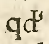
\includegraphics[height=06ex]{img/27a-1_Zaborowski_Polona03_quod}
    
\includegraphics[height=06ex]{img/27a-2_Zaborowski_Polona08_quod}
    \caption{On the left Capelli's dictionary, next Zaborowski's treatise (1518)}
    \label{fig:dzawijas}
  \end{figure}

  
\item [0xF0008] LATIN SMALL LETTER D WITH HIGH OVERLINE VARIANT:\\
  \Jglyph{󰀈}.\\ Cf. \url{https://github.com/psb1558/Junicode-New/discussions/44#discussioncomment-202860}.
\item [0xF0009] LATIN CAPITAL LETTER E WITH STROKE THROUGH TERMINAL VARIANT [JuniusX]:\\
  \Jglyph{󰀉}.\\ Cf. \url{https://github.com/psb1558/Junicode-New/issues/13}.
  
  In JuniusX font accessible also as \textit{E} with \texttt{cv08[2]};
  cf. \autocite[p. 7]{baker20:_opent_featur_junius_junius}.

 May be considered also as a variant of LATIN CAPITAL LETTER E WITH
 STROKE (U+0246).

 Occurs in particular in \textit{Nowe Ateny} (Supplement 1774,
 \url{http://www.wbc.poznan.pl/Content/6663/index.djvu?djvuopts=&page=1783.djvu},
 cf. Fig. \vref{fig:NA1774}.
 

  \begin{figure}[h]
    
\includegraphics[width=1.3\textwidth]{img/00435077wezach}
    \caption{\J W󰀉ZACH (1774)}
    \label{fig:NA1774}
  \end{figure}

 \item [0xF000A] LATIN SMALL LETTER E WITH STROKE THROUGH TERMINAL VARIANT [JuniusX]:\\
  \Jglyph{󰀊}.\\ Cf. \url{https://github.com/psb1558/Junicode-New/issues/13}.

  In JuniusX font accessible also as \textit{A} with \texttt{cv08[2]};
  cf. \autocite[p. 7]{baker20:_opent_featur_junius_junius}.

  For completeness it should be noted that there is also the variant
  \texttt{cv08[1]} of \textit{Ę} intended for the Latin abbreviation
  of \textit{AE}.

 Occurs in particular in \textit{List o oblężeniu zamku Dyjamenckiego} (1605,
 \url{https://cbdu.ijp.pan.pl/id/eprint/2910/},
 cf. Fig. \vref{fig:e1605}.
 
  \begin{figure}[h]
    
\includegraphics[width=1\hsize]{img/00436649jezyk}
    \caption{\J j󰀊zyk (1605)}
    \label{fig:e1605}
  \end{figure}

 May be considered also as a variant of LATIN SMALL LETTER E WITH
  STROKE (U+0247).

\item [0xF000B] LATIN SMALL LETTER F VARIANT [JuniusX]:\\
  \Jglyph{󰀋}.\\ % Cf. \url{https://github.com/psb1558/Junicode-New/issues/??}.
  In JuniusX font accessible also as \textit{f} with \texttt{cv09[5]};
  cf. \autocite[p. 9]{baker20:_opent_featur_junius_junius}.

  For completeness it should be noted that there is also the variant
  \texttt{cv08[1]} of \textit{ę} intended for the Latin abbreviation
  of \textit{ae}.
  
\item [0xF000C] LATIN SMALL LETTER I WITH HIGH OVERLINE VARIANT [JuniusX]:\\
  \Jglyph{󰀌}.\\ Cf. \url{https://github.com/psb1558/Junicode-New/discussions/44#discussioncomment-202860}.
\item [0xF000D] LATIN SMALL LETTER J VARIANT [JuniusX]:\\
  \Jglyph{󰀍}.\\ % Cf. \url{https://github.com/psb1558/Junicode-New/issues/??}.

  % In JuniusX font accessible also as \textit{đ}  (U+0111) with \texttt{cv06[1]};
  % cf. \autocite[p. 7]{baker20:_opent_featur_junius_junius}.
\item [0xF000E] LATIN SMALL LETTER J WITH HIGH OVERLINE  VARIANT [JuniusX]:\\
  \Jglyph{󰀎}.\\ Cf. \url{https://github.com/psb1558/Junicode-New/discussions/44#discussioncomment-202860}.
\item [0xF000F] LATIN SMALL LETTER L WITH HIGH ROUNDED STROKE VARIANT [JuniusX]:\\
  \Jglyph{󰀏}.\\  Cf. \url{https://github.com/psb1558/Junicode-New/issues/4}.
  In JuniusX font accessible also as \textit{ꝉ} (U+A749) with \texttt{cv17[1]};
  cf. \autocite[p. 9]{baker20:_opent_featur_junius_junius}.

  
\item [0xF0010] LATIN SMALL LETTER M WITH HIGH OVERLINE VARIANT [JuniusX]:\\
  \Jglyph{󰀐}.\\ Cf. \url{https://github.com/psb1558/Junicode-New/discussions/44#discussioncomment-202860}.
 \item [0xF0011] LATIN SMALL LETTER O WITH STROKE HORNED VARIANT [JuniusX]\\
  \Jglyph{󰀑}.\\  Cf. \url{https://github.com/psb1558/Junicode-New/issues/3}.
  In JuniusX font accessible also as \textit{ø} (U+00F8) with \texttt{cv21[1]};
  cf. \autocite[p. 9]{baker20:_opent_featur_junius_junius}.
\item [0xF0012] LATIN SMALL LETTER O WITH SHIFTED STROKE VARIANT [JuniusX]\\:
  \Jglyph{󰀒}.\\  Cf. \url{https://github.com/psb1558/Junicode-New/issues/3}.

  In JuniusX font accessible also as \textit{ø} (U+00F8) with \texttt{cv21[2]};
  cf. \autocite[p. 9]{baker20:_opent_featur_junius_junius}.
\item [0xF0013] LATIN SMALL LETTER O WITH STROKE HORN DOWNWARDS VARIANT [JuniusX]\\:
  \Jglyph{󰀓}.\\  Cf. \url{https://github.com/psb1558/Junicode-New/issues/3}.

  In JuniusX font accessible also as \textit{ø} (U+00F8) with \texttt{cv21[3]};
  cf. \autocite[p. 9]{baker20:_opent_featur_junius_junius}.
\item [0xF0014] LATIN SMALL LETTER O WITH STROKE HORN UPWARDS VARIANT [JuniusX]\\:
  \Jglyph{󰀓}.\\  Cf. \url{https://github.com/psb1558/Junicode-New/issues/3}.

  In JuniusX font accessible also as \textit{ø} (U+00F8) with \texttt{cv21[4]};
  cf. \autocite[p. 9]{baker20:_opent_featur_junius_junius}.
\item [0xF0015] ???  [JuniusX]\\:
  \Jglyph{󰀕}.\\%  Cf. \url{https://github.com/psb1558/Junicode-New/issues/3}.
\item [0xF0016] LATIN SMALL LETTER RUM ROTUNDA VARIANT [JuniusX]\\:
  \Jglyph{󰀖}.\\%  Cf. \url{https://github.com/psb1558/Junicode-New/issues/3}.

  In JuniusX font accessible also as \textit{ꝝ} (U+A75D) with \texttt{cv41[1]};
  cf. \autocite[p. 12]{baker20:_opent_featur_junius_junius}.
\item [0xF0017] LATIN SMALL LETTER V WITH LOW OVERLINE VARIANT [JuniusX]:// 
  \Jglyph{󰀗}.\\ Cf. \url{https://github.com/psb1558/Junicode-New/discussions/44#discussioncomment-202860}.
\item [0xF0018] LATIN SMALL LETTER V WITH HIGH OVERLINE VARIANT [JuniusX]:// 
  \Jglyph{󰀘}.\\ Cf. \url{https://github.com/psb1558/Junicode-New/discussions/44#discussioncomment-202860}.
\item [0xF0019] LATIN SMALL LETTER X WITH LOW OVERLINE VARIANT [JuniusX]:// 
  \Jglyph{󰀙}.\\ Cf. \url{https://github.com/psb1558/Junicode-New/discussions/44#discussioncomment-202860}.
\item [0xF001A] LATIN SMALL LETTER V WITH HIGH OVERLINE VARIANT [JuniusX]:// 
  \Jglyph{󰀚}.\\ Cf. \url{https://github.com/psb1558/Junicode-New/discussions/44#discussioncomment-202860}.
\item [0xF001B] LATIN LETTER GLOTTAL STOP VARIANT [JuniusX]\\
  \Jglyph{󰀛}.\\%  Cf. \url{https://github.com/psb1558/Junicode-New/issues/??}.
% \\item [0xF001C] LATIN SMALL LETTER RUM ROTUNDA VARIANT [JuniusX]\\:
\item [0xF001C] TIRONIAN SIGN CAPITAL ET VARIANT [JuniusX]\\:
\Jglyph{󰀜}.%\\%  Cf. \url{https://github.com/psb1558/Junicode-New/issues/??}.

In JuniusX font accessible also as \textit{⹒} (U+2E52) with \texttt{cv40[1]};
  cf. \autocite[p. 12]{baker20:_opent_featur_junius_junius}.

\item [0xF001D] TIRONIAN SIGN ET VARIANT [JuniusX]\\:
  \Jglyph{󰀝}.\\%  Cf. \url{https://github.com/psb1558/Junicode-New/issues/??}.
  In JuniusX font accessible also as \textit{⁊} (U+2E52) with \texttt{cv40[1]};
  cf. \autocite[p. 12]{baker20:_opent_featur_junius_junius}.

\item[0xF001E] LATIN CAPITAL LETTER A WITH STROKE
  VARIANT [JuniusX]: \Jglyph{󰀞}.\\
  Cf. \url{https://github.com/psb1558/Junicode-New/issues/14}.
  % The
  % term \textit{terminal} used after ???.\\
  
  In JuniusX font accessible also as \textit{A} with \texttt{cv02[2]};
  cf. \autocite[p. 7]{baker20:_opent_featur_junius_junius}.
% 
%  Used in particular in ???, cf. Fig. ???

    May be considered also as a variant of LATIN CAPITAL LETTER A WITH
  STROKE (U+023A).

  
\item [0xF001F] LATIN SMALL LETTER A WITH STROKE  VARIANT [JuniusX]: 
  \Jglyph{󰀟}.\\ Cf. \url{https://github.com/psb1558/Junicode-New/issues/14}.
  % The
  % term \textit{terminal} used after ???.

  In JuniusX font accessible also as \textit{A} with \texttt{cv02[2]};
  cf. \autocite[p. 7]{baker20:_opent_featur_junius_junius}.

  May be considered also as a variant of LATIN SMALL LETTER A WITH
  STROKE (U+2C65).

\end{description}

\printbibliography
\end{document}

– Nowe Ateny albo Akademia wszelkiey scyencyi pełna,
na różne tytuły iak na classes podzielona, mądrym
dla memoryału, idiotom dla nauki, politykom dla
praktyki, melancholikom dla rozrywki erygowana ...
/ przez Xiędza Benedykta Chmielowskiego ...
.
Część 1.2. http://www.wbc.poznan.pl/publication/3735,
publication date 1756??? (drugie wydanie), 844 pages.

Nowe Ateny, albo Akademia wszelkiey scyencyi pełna, na różne tytuły
iak na classes podzielona, mądrym dla memoryału, idiotom dla nauki,
politykom dla praktyki, melancholikom dla rozrywki erygowana
... . Część 3 albo Supplement.
Nowe Ateny, albo Akademia wszelkiey scyencyi pełna,
na różne tytuły iak na classes podzielona, mądrym
dla memoryału, idiotom dla nauki, politykom dla
praktyki, melancholikom dla rozrywki erygowana ...
. Część 3 albo Supplement.. http://www.wbc.poznan.
pl/publication/37543, publication date 1754, 741 pages.


DżZ. Zbiór rytmów duchownych Panegirycznych Moral- nych i
Swiatowych [...] Elżbiety z Kowalskich Druzback- iey [...] Zebrany y
do druku podany przez J. Z. R. K.  O. W. etc. [Załuskiego Józefa
Andrzeja]. http://www.wbc.poznan.pl/publication/13950, publication
date 1752, 566 pages.

List o oblężeniu zamku Dyjamenckiego w Inflantach do Krzysztofa Moniwida Dorohostajskiego, dnia 22 października 1605 pisany

http://cbdu.id.uw.edu.pl/2910/1/Z291.djvu?djvuopts=&page=0006l.djvu 

https://cbdu.ijp.pan.pl/id/eprint/2910/
%%% Local Variables: 
%%% coding: utf-8-unix
%%% eval: (set-fontset-font "fontset-default" '(#xF0000 . #xF001F) (font-spec :size 18 :name "JuniusX"))
%%% mode: latex
%%% TeX-master: t
%%% TeX-PDF-mode: t
%%% TeX-engine: xetex
%%% End: 
